			\documentclass{llncs}
				\usepackage{llncsdoc}
				\usepackage[noend]{algpseudocode}
				\usepackage{subfig} 
				\usepackage{graphicx}
				\usepackage{frame, caption}
				\usepackage{amsmath}
				\usepackage{eulervm}
				\usepackage{fontenc}
				\usepackage{mathrsfs}
				\usepackage{multirow}
				\usepackage{array}
				\usepackage[rflt]{floatflt}
				\usepackage{makecell}	
				\usepackage{xcolor, soul}
				\sethlcolor{yellow}	
				\usepackage{floatrow}
				% Table float box with bottom caption, box width adjusted to content
				\newfloatcommand{capbtabbox}{table}[][\FBwidth]
				
				\begin{document}
						\title{\vskip -10pt Dominance in dialogue of cooperative negotiation}
						\maketitle
					\section{Introduction}
					Dialogue systems are artificial systems capable to hold a conversation with a human user, usually to achieve certain objective or fulfill a task.
					% Existing conversational agents provided with dialogue system play different roles like 
					
					During a human-human dialogue, interlocutors establish a social relationship that affect their behaviors. Previous researches have shown that people tend to respond to computers as social actor [bickmore], which lead the community to assess the psychosocial relationship between the person and the agent during their interaction. 
					A growing body of research is investigating the use of appropriate social behavior for virtual agents in different roles and types of user-computer relationship.
					For example, Bickmore studied the impact of trust ...[To complete]
					
					
					In this paper, we are interested in modeling a dialogue system for social dialogue in which user and agent cooperate in order to achieve a common objective.  We believe that individuals that collaborate to fulfill an objective (for example: find a restaurant for dinner), have their own preferences in the way to do it, which lead them to conduct a \emph{cooperative negotiation} about their preferences in order to determine a trade-off that satisfy both interlocutors. Moreover, scholars in social psychology and communication investigated the impact interactive effects of relations and emotion in negotiation, and proved that  \emph{interpersonal dominance} affect the strategies of negotiators. Our objective is to build an agent that can perceive the established relation of dominance and adapt its strategy of negotiation to the relation. 
					
					In the next section, we review related works on designing social agents. Section 3 will relate our definition of dominance based on research on social psychology. In section 4, we present our model of dialogue. Section 5 will discuss our experiment and the analysis obtained results. 
				
					
					\section{Dominance in dialogue}
					\par Despite the various definitions of dominance available in the fields of interpersonal communication and psychology, scholars are converging to a general definition of dominance as the power to produce intended effects, and the ability to influence the behavior of other person in the conversation. \cite{dunbar2005perceptions}. Dominance is generally viewed as a personality trait, or to describe the social role of an individual inside a group. However, in the context of communication, dominance is a dyadic variable where one individual's attempt of control is necessarily acquainted by the partner in the interaction.\cite{dunbar2005perceptions}. 
					\par Dominant behaviors in a conversation can contribute either positively or negatively to the discussion. For example, positive contributions include actions such as keeping the conversation going, orient the task decision, by making quick decisions and conclusions etc. Negative contributions may include not considering the partner in the conversation, for example, not giving the occasion to express his opinion, not open to criticism. In addition, expressing verbally the dominance can be viewed as offensive and unjustified \cite{zablotskaya2012relating}. Giving these contributions to the conversation, several researches get interested to detect behaviors related to the dominance during the conversation. We focus essentially on the context of conversation of negotiation, where several researches already proved the impact of dominance on the negotiation\cite{van2006power}.
					
					\subsection{Behaviors of dominance in dialogue}
					Several scholars studied behaviors related to the dominance in order to gain a better understanding to social relations. During a conversation, dominance can be perceived through verbal and nonverbal behaviors. We present in this section behaviors related to dominance that can be perceived in a conversation of cooperative negotiation.
					\subsubsection{Non-verbal behaviors:}
					At the non-verbal level, a wide range of behaviors have been associated with dominance. \cite{burgoonnonverbal} divide non-verbal behaviors into classes such (kinesics, vocalic, ). First, kinesics behaviors are considered as the richest of all the codes that includes facial expression, body movements, gestures. Indeed, dominant individuals are related with high visual ratio (high looking while speaking / listening).  Furthermore, \cite{burgoonnonverbal} found that the more body control an individual had the more observers perceived her as dominant. In addition, dominant individuals are more susceptible to use gesture when they talk.  
					\par  Second, voice cues of dominance manifest by speaking duration, speaking intensity, voice control and pitch. Dominant individuals speak loudly and more frequently and might cause interruption while other are talking \cite{dunbar2005perceptions}.
					
					\subsubsection{Verbal behaviors:}
					verbal behaviors of dominance in the dialogue are related to the type of \textit{strategies} that individuals choose in order to take control of the other especially during a negotiation. Therefore, dominant negotiators tend to end up with the larger share of the pie \cite{giebels2000interdependence}. 
					\par A considerable body of research has documented the effects of dominance on negotiation behaviors and outcomes. First, in De Dreu researches about the impact of social value orientation in negotiation strategies, he demonstrated that \cite{de1995impact} dominant negotiators have higher aspirations, demands more and concede less. 
					
					 Moreover, Galinsky \cite{galinsky2003power} affirms that the dominance increases the action orientation. Dominant negotiators control the flow of the negotiation. In addition, dominant behavior increase task orientation and goal-directed behavior. In addition, Dominance affects the way that negotiators gather information about their partners. Negotiators with less power have a stronger desire to develop an accurate understanding of their negotiation partner, which would lead them to ask more \emph{diagnostic} rather than \emph{leading} questions.
					 
					 Furthermore, it was shown \cite{fiske1993controlling},\cite{de1995impact} that dominant negotiators are self-centered and tend to not pay attention to submissive negotiators .
%					 The idea is that high-dominant individuals have many resources and can often act at will without serious consequences, while submissive individuals, have to be more careful because they are more dependent on other people. In addition, they are motivated to gain or regain control over their outcomes by paying close attention to the people on whom they depend.
%					
					\par We are interested in this paper to the verbal behaviors for two main reasons. First, verbal behaviors are directly related to \emph{the strategies} deployed during the negotiation. In addition our dialogue system is text oriented, which make the non-verbal behavior impossible to reflect during the dialogue. 
					We present in the next section the decision model based on dominance behaviors. 
					
					\subsection{Principles of dominance in negotiation}
					Based on psychology research, we selected three main principles of behaviors in order to implement our conversational agent.
					\subsubsection{Principle 1: Self Vs Other}
						Submissive negotiators consider the prefereces of other in the negotiation, whereas dominant negotiators  are self-centred and only interested by satifying their own preferences.
					
					\subsubsection{Principle 2: Representation of demands}
					
%					Dominant negotiators adopt different strategies comparing to less powerful negotiators. Several researches in social psychology defined a panel of different behaviors in a negotiation:
%					
					 Dominant negotiators show a higher level of demand than the submissive ones. In addition,  Submissive negotiator's demand decrease over time, and tends to make larger concessions than dominant negotiators.
						
					
					
					\subsubsection{Principle 3:Control the flow of the negotiation}

						Dominant negotiators tend to make the first move \cite{magee2007power}. In addition, they take the lead of the negotiation.
						
%						\item Based on Carsten, De Dreu and Van Kleef demonstrate that high power negotiators are high in their propensity to negotiate relative to participants with low power. (leading individuals to focus on the rewards available to them in situations and to bargain forgreater rewards than were initially offered to them.)			
						

	\section{Model of negotiation based on dominance}
			%		
			%			 \subsection{Model of preferences}
			%			  \subsection{Model of communication}
			%			  \subsection{Strategies of negotiation (decision)}
				\subsection{Domain model}
				Consider a sequence of criterion sets $C_1, C_2, ..., C_n$ and an options set defined as the cross-product:
				$O = C_1 \times C_2 \times \ldots C_n$.
				
				For example, for restaurants, the criteria might be: \\
				Cuisine = \{Chinese, French, ...\} \\
				Cost = \{cheap, expensive, ...\} \\
				Atmosphere = \{quiet, lively, ...\} \\
				
				\par and a restaurant options might be: 
				\begin{itemize}
					\item $[Chinese, cheap, lively]$. 
					\item $[Chinese, expensive, quit]$.   
					\item $[Chinese, expensive, lively]$.
%					\item $[French, cheap, quit]$.  
%					\item $[French, expensive, quit]$.   
%					\item $[Chinese, expensive, lively]\ldots$ 
				\end{itemize}
				
				
				\subsection{Self model} 
				
				\subsubsection{Preferences for self}
				Preferences are partial orders (transitive, asymmetric binary relations) on the criterion sets. The preference relation on the criterion set $C_i$ is denoted by $\prec_i$.			
				Let $\prec$ denotes the sequence of preferences $\{ \prec_i, \prec_2, ..., \prec_n\}$
				
				\subsubsection{Self satisfaction function} 
				
				Satisfaction is a function normalized to [0,1] that evaluates an element of a criterion set relative to the corresponding preference relation, defined as follows.
				
				For $c \in C_i$ and $\prec_i$:
				
				$$sat(c, \prec_i) =	1 - \left( \frac{|\{d : d \neq c \  \wedge \ (c \prec_i d)\}| }{( |C_i| - 1 )}\right)  $$
				
				Satisfaction is generalized to options as a weighted sum.
				For $o \in O$ and where $o_i$ is the i-th element of $o$ and $\prec_i$ the i-th element of $\prec$.
				
				$$sat(o, \prec) = \frac{\sum_{i}^{n} sat(o_i, \prec_i) }{n} $$
				
				
				\subsection{Dialogue model}
				We present in the section the knowledge that the agent gather and processed from the dialogue.
				
				\subsubsection{Other model}
				We do not have detailed knowledge of the preferences of the other; the agent only knows which criteria values the other has said are acceptable or unacceptable.
				
				Let the collection of $A_i \subseteq C_i$ be the criterion values that are acceptable to the other, and $U_i \subseteq C_i$ be the criteria values that are unacceptable.  We assume $A_i \cap U_i = \emptyset$.  Note	that some values are thus unknown.
				
				Then the acceptability of a criterion $c \in C_i$ is a function normalized to [0,1] and defined as follows.
				$$ other(c, A_i, U_i)= \left\{\begin{array}{ll}
				1	 & \mathrm{if\ }  c \in A_i\\
				0    & \mathrm{if\ }c \in U_i\\
				0.5	 & \mathrm{otherwise}
				\end{array}\right.$$
				This function is generalized to options as a weighted sum.
				
				$$other(o, A, U) = \frac{ \sum_{i}^{n} other(o_i, A_i, U_i) } {n}$$ 
				
				\subsubsection{Negotiation state}
				During a negotiation, negotiators express two types of utterances: %that we name \emph{statement moves} and \emph{negotiation moves}. 
				
				\begin{itemize}
					\item \emph{Statement move:} Speaker share information about its preferences (StatePreference) or ask other about his preferences (askPreferences).
					\item \emph{Negotiation move:} Interlocutors negotiate about the different options of a topic (Propose, accept or reject proposals).
				\end{itemize}
				
				
				In order to produce coherent dialogues, the agent keeps track about the different states of the dialogue, that each move updates. 
				
				The negotiation might focus on each criterion of the discussed topic. For example, in a negotiation on restaurants, speakers might negotiate about the type of \textit{cuisine}, and the \textit{ambiance} to choose.  We note $D$ the set of criteria which have been discussed during the dialogue. When speakers agree on a value of a criterion to choose, the negotiation on this criterion is considered as \textit{closed}. We note $Cl$ the set of closed criteria.
				
				For each discussed criterion $C_i \in D$, the agent register the following information:		
				\begin{itemize}
					\item Let the collection of $S_i \subset C_i$ be the criterion values stated by the agent in the dialogue.
					\item Proposals which are made during the negotiation by both negotiators might have different status. They can either be accepted or rejected with respect of the decisional model (See section \ref{decision}).
					\subitem - $P_i$ is the set of  values which have been proposed in the negotiation.
					\subitem - $T_i$  is the set of values which have been accepted in the negotiation.
					\subitem - $R_i$  is the set of values which have been rejected in the negotiation.
				\end{itemize}
				
				Moreover, interlocutors are allowed to make proposals of options. Therefore we define the same structure of proposals for the options; $P, R, T$
				
				\subsection{Decision based on dominance in negotiation}
				\label{decision}
				\subsubsection {Dominance and concession}
				Let  $dom \in [0, 1] $ denotes the dominance of an agent (self) in the relationship.  It is a constant for a given agent in a given relationship.
				
				The weight that an agent gives to its self-satisfaction relative to	the satisfaction of the other is a time-varying function normalized to 	[0,1] of its dominance, defined as below.
				$$self(dom, t) = \left\{\begin{array}{ll}
				dom & \mathrm{if\ } (t \leq \tau)\\
				max(0, dom - (\frac{\delta}{dom} . (t - \tau))) & \mathrm{otherwise}
				\end{array}\right.$$
				
				
				where is $t \geq 0$ is the number of open or rejected proposals.
				
				This is called the "concession curve", where $\tau > 0$ and $\delta > 0$
				are parameters of the theory in general and are initially assumed to
				be 2 and 0.1, respectively.
				
				Therefore, the acceptability of a value $c \in C$  is relative to the weight an agent gives to its self satisfaction:
				
				$$acc(c, t) = sat(c, \prec_i) \geq  \beta \times Self(t)$$
				with $\beta > 0 $.
				
				This function is generalized to options:
				$$acc(o, t) = sat(o, \prec) \geq  \beta \times Self(t)$$
				
				
				\subsection{Lead of the negotiation}
				
				
				\subsubsection{Choosing an utterance type}
				Let $V$ be the set of available options (values), such that option :$ V\rightarrow O$	i.e., each value is a "name" for an option.  For example, V is the set of restaurants that are mutually known to the participants. This can be a many-to-one function, e.g., there could be two restaurants with same criteria.		
				
				We present in the following the possible responses and their applicability conditions. Note that each line (utterance)  assumes that the previous ones are already not applicable.
				
				$ chooseUtterance(dom, t, V, \prec, A, U) = $ \\
				
				
				\textbf{if(\textbf{dom  $>\sigma$})} 
				\begin{table}
				\centering
			
				\begin{tabular}{|p{3cm}|p{9cm}|}
					\hline
					\textbf{Utterance type} & Condition \\
					\hline
					Negotiation success & $\exists o \in T$   \emph{OR} $o \in P$ such that  $acc(o,t) = true$ \\
					\hline
					Negotiation failure & $ \forall o \in O$,  $o \in O$  \emph{OR} $acc(o,t) = false$\\
					\hline
					State & $type(u^{-1}) = AskPreference$  \textit{ and }
					$n < \alpha$ (with $n$ the number of successive statement moves)\\
					\hline
					AcceptPropose & $\exists c \in P_i$ / $acc(c,t)= true$ \\
					\hline
					RejectPropose & $\exists c \in P_i$ / $acc(c,t)= false$ \\
					\hline
					Propose & Otherwise  \\
					
					\hline
				\end{tabular}
				\end{table}
		
				
				\textbf{if(\textbf{dom  $ \leq \sigma$})} 
				\begin{table}
					\centering
				\begin{tabular}{|p{3cm}|p{9cm}|}
					\hline
					\textbf{Utterance type} & Condition \\
					\hline
					Negotiation success &  $\exists o \in T$ \\
					\hline
					Accept & $\exists c \in P_i$, $acc(c, t)=true $ \newline \emph{OR}   \newline $ \exists o \in P$ ,  $acc(o, t) =true$ \\
					\hline
					RejectState & $ [\exists c \in P_i$, $acc(c, t)= false $  \emph{OR}   $ \exists o \in P$ ,  $acc(o, t)=false]$ \newline  \emph{AND} $t<\tau$.\\
					\hline
					Propose & $\exists c$ / $other(c, A_i, U_i)  = 1 $  \emph{and}
					\newline $acc(c, t)=true$
					\newline \emph{OR}  
					\newline $\forall c \in C_i$,  $c \in T_i$\\
					\hline
					Ask &  \textbf{(}$t> \tau,$ \emph{and} 
					$\exists c \in P_i /$
					$ acc(c, t)=false$\textbf{) }
					\newline \emph{OR}
					\newline $ \forall c \in C_i,other(c, A_i, U_i)=0.5$ \\
					\hline
					
					State & $type(u^{-1}) = AskPreference$
					\newline \emph{OR}
					\newline $\exists x,other(x, A_i, U_i) \not = 0.5 $ 
					\newline \emph{OR}
					\newline $ \exists C \in \mathcal{C}, A_i(C) = Unkown$
					\\
					\hline
					Propose & Otherwise \\
					\hline
				\end{tabular}
					\end{table}
				
				\subsubsection{Choosing a value for an utterance} 
				
				
				Let be $\{V' \subset V$ / $\forall v \in V'$ $ acc(v,t) = true\}$ be the list of agent's acceptable values. 
				
				The value for a proposal should be tolerable for both interlocutors. Therefore,  in addition to self preferences, the agent should considers other preferences. 
				
				We define a tolerance function of a criterion $c \in C_i$ as a function normalized to [0,1] and defined as below.
				
				$$tolerable(dom, t, c, \prec, A, U) = self(dom, t) . sat(c, \prec_i) \ +\  (1 - self(dom, t)) . other(c, A_i, U_i)$$
				
				Tolerance is generalized to options as a weighted sum.
				
				$$tolerable(dom, t, o, \prec, A, U) = \frac{ \sum_{i}^{n} tolerable(dom, t, o_i, \prec_i, A_i, U_i) } {n}$$ 
				
				
				
				The following function returns the most tolerable element of $V'$ to make a proposal.
				
				$$ chooseValue(dom, t, V, \prec, A, U) =	\operatorname*{arg\,max}_{name \in V} tolerable(dom, t, option(name), \prec, A, U) $$
				
				Note that argmax may not be unique.  The following function returns the most tolerable element of	criterion $C_i$.
				
				$$chooseCriterion(dom, t, V, \prec, A, U, C_i) = option(chooseValue(dom, t, V, \prec, A, U, C_i))_i$$
				
				
				
				
				\subsection{Summary of general parameters }
				\begin{itemize}
					
					\item $\sigma \in $[0,1] : boundary between submissive and dominant used in
					choosing an utterance type
					%		\item $\beta$:  a value that represent the minimum score that a value has to get to be positively satisfiable to the agent preferences in the negotiation. Note that $\beta = const \times self(dom,t)$.
					\item $\tau > 0$ : the minimum number of open or rejected proposals before.
					concession begins
					\item $\delta > 0$ : parameter in slope of concession curve.
					\item $u^{-1}$ refers to the previous utterance.
					\item $\alpha> 0$: the maximum number of successive statement moves.
					
					
				\end{itemize}
				
			
						  
				\section{Evaluation}
				
				 We built a conversational agent able to deploy a strategy of negotiation based on its perception of interpersonal relationship of dominance. 
				 
				 In order to validate our model, we conducted a perceptual study in which participants have to determine the behaviors of two agents generated using our model. 
				 
					\subsection{Study design}
			%	We developed an experimental scenario in which we generated dialogues of negotiation between two agents implemented with the proposed model. We used a social topic of "negotiation about a restaurant where to have dinner".
				We used our model to develop two conversational agents which have to negotiate about a social topic of "negotiation about a restaurant where to have dinner".
				
				We generated a set of dialogues where we manipulated two main conditions. First, the initial value of the dominance \textbf{dom} (see section \ref{decision}). The purpose was to define the behavior of agents in negotiation.
				We aimed to make the first agent \emph{(Agent 1)} adopt more a dominant behavior by initiating the value of its dominance \textbf{dom} in the higher range of the dominance spectrum ($dom>\sigma$). Complementarity, the second agent \emph{(Agent 2)} had to adopt a submissive behavior. Therefore we initiated its \textbf{dom} to be in the lower range. ($ dom\leq \sigma$).
				
				The second condition involved varying the initial preferences of both agents. We manipulated the initial preferences to be either \textit{similar} or \textit{different}. We used the metric of Kendall distance \cite{bra2013Kendall} in order to compute the distance between two preferences sets (see section \ref{decision}).  
				We figured out, that the dialogues generated with the \textit{similar} preferences condition are quite similar, because the negotiation converges quickly. Therefore, we presented only one dialogue in the \textit{similar preferences} condition for the experiment. 
				The conditions manipulated to generate the dialogues are depicted in table \ref{Conditions}
				
				
			\begin{table}
				\label{Conditions}
				\centering
		\begin{tabular}{ |l|c|c|l| }
					\hline
					\multicolumn{3}{ |c| }{Conditions} & \multirow{2}{*}{Dialogue's label}  \\ \cline{1-3}
		
					\newline \multirow{2}{*} {\textbf{Initial preferences}}& \multicolumn{2}{ |c| } {\textbf{Dominance}} & \\ \cline{2-3}
		
					\newline  & dom(Agent 1) & dom(Agent 2) &  \\ 
					\hline
					 \newline\multirow{3}{*} {Different preferences} & 0.9 & 0.4 & Dialogue 1 \\ \cline{2-4}
					 
					 \newline  & 0.7 & 0.4 & Dialogue 2\\ \cline{2-4}
					 
					 \newline   &0.7 & 0.2 & Dialogue 3\\ 
					 \hline
					 \newline Similar preferences & 0.7 & 0.4 & Dialogue 4\\
					 \hline
				\end{tabular}
				\caption{Initial condition's setting for generating dialogues}
			\end{table}
				
		
				
			%	We present in table the initial setting for agents for the presented dialogues in the experiment.
				
						
				\subsection{Hypotheses}
				 We investigated four main hypotheses about the perception of agents behaviors of dominance during the negotiation. 
				 \begin{itemize}
				 	\item  \textbf{H1:} In the dialogue, the speaker with the higher dominance will more strongly be perceived as self-centered.  
				 	
				 	\item \textbf{H2:} The speaker with the lower dominance is more strongly perceived as making concessions.
				 	
				 	\item \textbf{H3:} The speaker with the higher dominance is perceived as having a higher level of demand comparing to the speaker with a lower dominance.
				 	
				 	\item \textbf{H4:} The speaker with the higher dominance is more strongly perceived as taking the lead of the negotiation.
				 	
				 \end{itemize}
						
				\subsection{Experimental Procedure}
				
				We conducted a between-subject study using an online crowdsoursing website \emph{CrowdFlower} \footnote{https://www.crowdflower.com/}. 
				
				%Each generated dialogue had a questionnaire. There were 12 questions (including 2 test questions).
				
				Each participant was shown only one dialogue, where the task was to judge each agent behaviors. Agents were described as two friends (Speaker A as Agent1, Speaker B as Agent2) trying to find a restaurant where to have dinner. We wanted to avoid skewing the participant's perception by the fact that negotiators are artificial agents. Participants were invited to read the assigned dialogue and answer the corresponding questionnaire. 
				
				We defined for each hypothesis two questions (asked for both speakers) to analyze the speaker's behaviors related to the hypothesis. 
				Two test questions were included to check the sanity of the answers. Therefore, the questionnaire was defined with 18 questions.
				
				\subsection{Participants}
				A total of 120 subjects participated to the experiment. They were recruited through the website \emph{Crowdflower.com}, for which each subject received \textit{25 cents}. 
				
				We limited the participant pools to native English speakers. We excluded participants providing wrong answers to our sanity questions. The final number of accepted participants was 105. 
				
				\subsection{Results}
				 In order to analyze participant's responses, we computed the correlation for each pair of questions of the same hypothesis. The obtained results showed a high correlation between each pair of questions for all the hypotheses.
				
				The obtained data was analyzed using a non parametric test, and all pairwise comparison of of agent 1 and agent 2 behaviors were analyzed using Wilcoxon signed-rank test for paired data. All the results are resumed in the tables in the Appendix.
				
				\par Our first hypothesis (H1) stated that participants would perceive agents with the higher dominance to be self-centered and only care about their own preferences. Our analysis confirmed our prediction. For example, results obtained for \textit{dialogue2} showed that in average Agent1 was perceived as more self-centered (M=3.6, SD=0.9) than Agent 2 (M=2.2, SD=0.8) and (\textit{p$<$0.01}). The same results were observed for all the dialogues. Theses results are depicted in figure \ref{H1}.
				
				\par Our second hypothesis (H2) predicted that agents with the lower dominance will be perceived to make larger concessions. For all the proposed dialogues, participants responses supported our hypothesis. 
				For instance, in \textit{dialogue 1} participants reported that Agent2 made larger concessions (M=4.3, SD=0.8), than did the Agent 1(M=2.19, SD=1.1), (\textit{p$<$0.01}).  (see figure  \ref{H2})
				
							\begin{figure}[htb!]
					\setlength\fboxsep{0pt}\setlength\fboxrule{0.75pt}
					\ffigbox[\textwidth]
					{
						\begin{subfloatrow}[2]
							%\fbox{
							\ffigbox[.49\textwidth]
							{
								\caption{Results of hypothesis H1}
								\label{H1}
							}
							{
								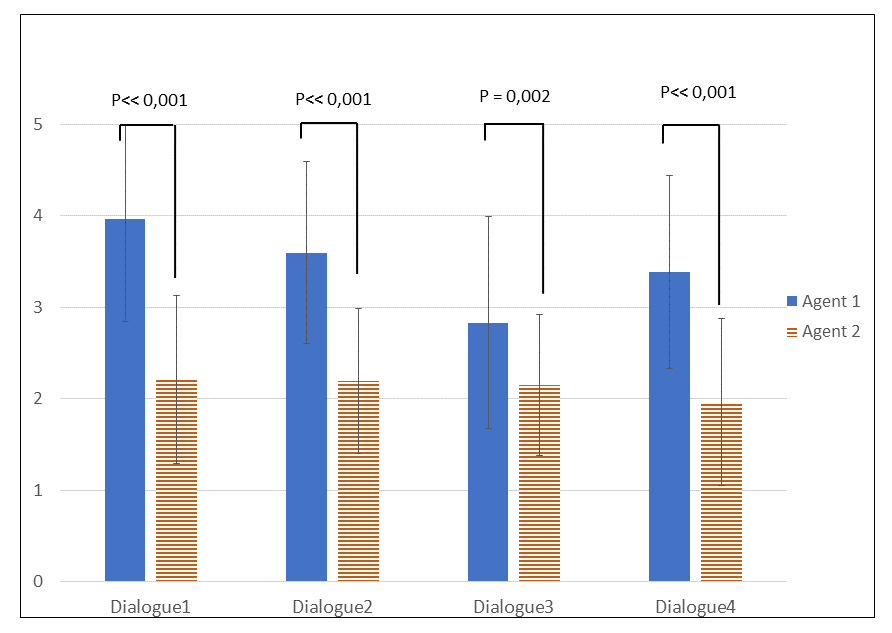
\includegraphics[width=.7\linewidth]{graphs/H1}%
							}
							%}
							%\fbox{
							\ffigbox[.49\textwidth]
							{
								\caption{Results of hypothesis H2}
								\label{H2}
							}
							{
								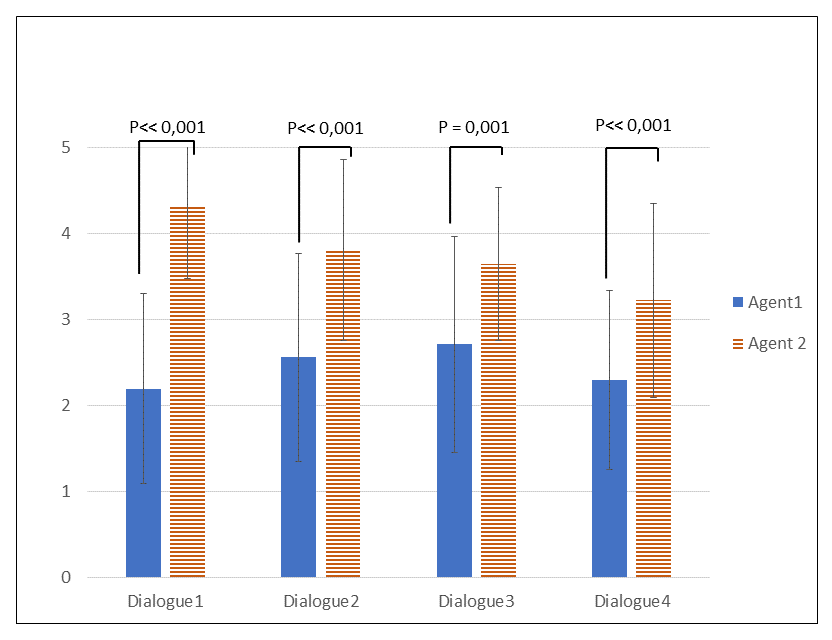
\includegraphics[width=.7\linewidth]{graphs/H2}%
							}
							%}
						\end{subfloatrow}%
					}
					{
						\caption{Results of H1 and H2}
						
					}
				\end{figure}%
				
				\par The third hypothesis was also supported in all the dialogues. H3 stated that agents with the higher dominance in dialogue are more strongly perceived as having higher level of demand. As can be seen in Figure \ref{H3} , in all the dialogues, Agent 1 was perceived as expressing a higher level of demand than Agent 2 does. For instance, in dialogue 1, the level of demand was rated for Agent 1(M=4.07, SD = 0.8) versus Agent 2(M= 2.65, SD =1.1), with a \textit{p-value $<$ 0.01}.
				
				\par Finally, for the last hypothesis H4, the analysis revealed a significant main effect of the dominance in the lead of the dialogue, indicating that participants perceived agents with the higher dominance (Agent 1) as more leading the dialogue than agents with lower dominance (Agent2). In dialogue 1, participants indicated that Agent 1 is the one who leads the dialogue (M=4.2, SD=0.8) comparing to Agent 2 (M=2.3, SD= 1.1), \textit{p$<$ 0.01}. These results are depicted in the figure \ref{H4}.
				
			\begin{figure}[htb!]
				\setlength\fboxsep{0pt}\setlength\fboxrule{0.75pt}
				\ffigbox[\textwidth]
				{
					\begin{subfloatrow}[2]
						%\fbox{
						\ffigbox[.49\textwidth]
						{
							\caption{Results of hypothesis H3}
							\label{H3}
						}
						{
							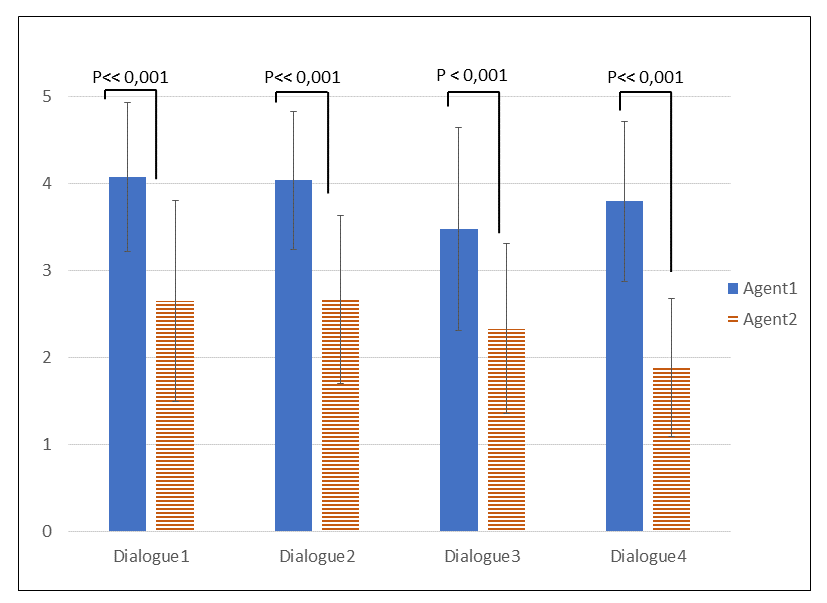
\includegraphics[width=.7\linewidth]{graphs/H3}%
						}
						%}
						%\fbox{
						\ffigbox[.49\textwidth]
						{
							\caption{Results of hypothesis H4}
							\label{H4}
						}
						{
							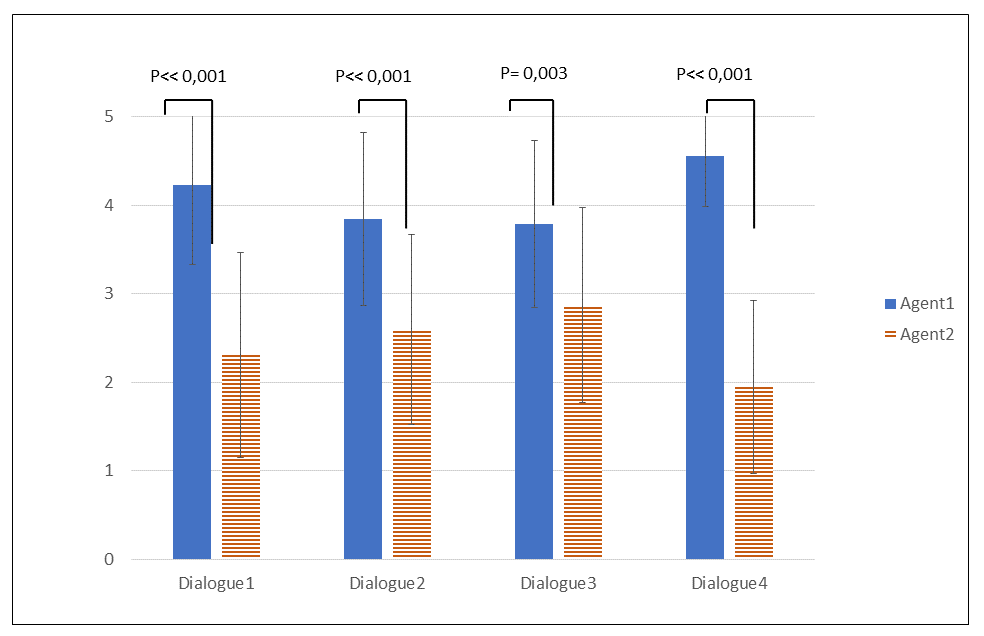
\includegraphics[width=.7\linewidth]{graphs/H4}%
						}
						%}
					\end{subfloatrow}%
				}
				{
					\caption{Results of H3 and H4}

				}
			\end{figure}%
			 \subsection{Discussion}

			 our research aims to model a conversational agent which is able to deploy strategies of negotiation in function of its representation of dominance. Our on-line study had the purpose to validate the implemented behaviors and did provide strong support to the claim that the relation of dominance affects agent's behaviors in negotiation.
			 
			 We found that participants perceived a significant difference in the agent's behaviors depending on their respective relation of dominance.  
			 Indeed, all of our four hypotheses were confirmed. We predicted that agents with higher dominance will be perceived as more individualist and self-centred, whereas agents with lower dominance would care about other preferences. Furthermore, agents with lower dominance were perceived to make larger concessions than did agents with higher dominance. Consistent with this prediction, agents with higher dominance showed a greater level of demand in the negotiation. Finally, we obtain evidence that agents with higher dominance tends to lead the dialogue and take control of the negotiation's flow. 
			 
			 In addition to theses finding, we extended our analysis to understand the perception of dominance in dialogue.
			
			 First, we studied the influence of the initial preferences in the generation and perception of behaviors of dominance.
			 We supposed that when the initial preferences of agents are similar (\textit{similar preferences} condition), behaviors related dominance won't be perceived due to the high aspect of cooperation in the negotiation. However, as our results demonstrated for dialogues generated in the similar preferences condition, (see results of Dialogue 4), all the hypotheses were supported even when the preferences were quiet similar. Therefore, the behaviors of dominance implemented are not affected by the initial preferences of agents.
			 
			 Second, we get interested in analyzing the behaviors of dominance in the spectrum of dominance. We supposed that the highest the dominance gets in the spectrum, the better behaviors of dominance will be perceived. We did compare participant's judgments of Agent 1 in dialogues where Agent 1 had different setting of dominance whereas Agent 2 had the same setting. We specially compared Agent1 behaviors in Dialogue 1 and Dialogue 2. The results obtained are presented in the figure ... 
			 
			 Unfortunately, this hypothesis was not supported. We did not observe any significant difference in agents behaviors. This might be explained by the interpersonal nature of dominance, which means that participants rated the dominance of Agent 1 in opposition of Agent2, which makes the comparison in this case irrelevant. 
			 
			 \par  The results presented have a number of limitations. Participants judged the dialogues from an external point of view which might influence the engagement in the process of judging agent behavior. The next step, would be to experiment our model with an interaction with humans. Moreover, we aim to to extend our model with a module of theory of mind that would allow the agent to adapt its behavior to complement the user behavior perceived during the dialogue.
			 
			 
			 \section{Related works}			
			 	
			 \section{Conclusion and future works}
			 
			 \section{Appendix}
			 	\begin{table}
			 	\label{ref-H1}
			 	\begin{tabular}{l|c|c|c|c|c|c|c|c|} 
			 		\cline{2-9}
			 		
			 		\newline \multirow{2}{*} {}	&\multicolumn{2}{c|} {Dialogue1} & \multicolumn{2}{c|} {Dialogue2} & \multicolumn{2}{c|} {Dialogue3} &\multicolumn{2}{c|} {Dialogue4} \\ \cline{2-9}
			 		
			 		
			 		\newline & Agent1 & Agent2 & Agent1 & Agent2 & Agent1 & Agent2 & Agent1 & Agent2 \\
			 		\hline 
			 		
			 		\multicolumn{1}{|l|}{ \textit{Mean} $\pm$ \textit{SD} } & 3.9 $\pm$ 1.1 & 2.2$\pm$ 0.9  & 3.6 $\pm$0.9 & 2.2 $\pm$0.8  &2.8 $\pm$1.1  & 2.13$\pm$ 0.7 & 3.4 $\pm$ 1 & 2 $\pm$0.9 \\
			 		\hline	
			 		\multicolumn{1}{|l|}{p-value} & \multicolumn{2}{c|}{ $<<0.01$} & \multicolumn{2}{c|}{ $<<0.01$} & \multicolumn{2}{c|}{ $<0.01$}& \multicolumn{2}{c|}{ $<<0.01$}\\
			 		\hline	
			 	\end{tabular}
			 	\caption{Results of H1}
			 \end{table}
		 
		 \begin{table}
		 	\label{ref-H1}
		 	\begin{tabular}{l|c|c|c|c|c|c|c|c|} 
		 		\cline{2-9}
		 		
		 		\newline \multirow{2}{*} {}	&\multicolumn{2}{c|} {Dialogue1} & \multicolumn{2}{c|} {Dialogue2} & \multicolumn{2}{c|} {Dialogue3} &\multicolumn{2}{c|} {Dialogue4} \\ \cline{2-9}
		 		
		 		
		 		\newline & Agent1 & Agent2 & Agent1 & Agent2 & Agent1 & Agent2 & Agent1 & Agent2 \\
		 		\hline 
		 		
		 		\multicolumn{1}{|l|}{ \textit{Mean} $\pm$ \textit{SD} } & 2.2 $\pm$ 1.1 & 4.3$\pm$ 0.8  & 2.5 $\pm$1.2 & 3.8 $\pm$1.04 &2.7 $\pm$1.2  & 3.6$\pm$ 0.8 & 2.3 $\pm$ 1 & 3.2 $\pm$1.2 \\
		 		\hline	
		 		\multicolumn{1}{|l|}{p-value} & \multicolumn{2}{c|}{ $<<0.01$} & \multicolumn{2}{c|}{ $<<0.01$} & \multicolumn{2}{c|}{ $=0.01$}& \multicolumn{2}{c|}{ $<<0.01$}\\
		 		\hline	
		 	\end{tabular}
		 	\caption{Results of H2}
		 \end{table}
	 
	 
	 		 \begin{table}
	 	\label{ref-H1}
	 	\begin{tabular}{l|c|c|c|c|c|c|c|c|} 
	 		\cline{2-9}
	 		
	 		\newline \multirow{2}{*} {}	&\multicolumn{2}{c|} {Dialogue1} & \multicolumn{2}{c|} {Dialogue2} & \multicolumn{2}{c|} {Dialogue3} &\multicolumn{2}{c|} {Dialogue4} \\ \cline{2-9}
	 		
	 		
	 		\newline & Agent1 & Agent2 & Agent1 & Agent2 & Agent1 & Agent2 & Agent1 & Agent2 \\
	 		\hline 
	 		
	 		\multicolumn{1}{|l|}{ \textit{Mean} $\pm$ \textit{SD} } & 4.1 $\pm$ 0.8 & 2.6$\pm$ 1.1  & 4.03 $\pm$ 0.8 & 2.7 $\pm$0.9 &3.5 $\pm$1.1  & 2.3$\pm$ 1 & 3.8 $\pm$ 1.8 & 1.8 $\pm$0.8 \\
	 		\hline	
	 		\multicolumn{1}{|l|}{p-value} & \multicolumn{2}{c|}{ $<<0.01$} & \multicolumn{2}{c|}{ $<<0.01$} & \multicolumn{2}{c|}{ $<0.01$}& \multicolumn{2}{c|}{ $<<0.01$}\\
	 		\hline	
	 	\end{tabular}
	 	\caption{Results of H3}
	 \end{table}
 
 
 		 \begin{table}
 	\label{ref-H1}
 	\begin{tabular}{l|c|c|c|c|c|c|c|c|} 
 		\cline{2-9}
 		
 		\newline \multirow{2}{*} {}	&\multicolumn{2}{c|} {Dialogue1} & \multicolumn{2}{c|} {Dialogue2} & \multicolumn{2}{c|} {Dialogue3} &\multicolumn{2}{c|} {Dialogue4} \\ \cline{2-9}
 		
 		
 		\newline & Agent1 & Agent2 & Agent1 & Agent2 & Agent1 & Agent2 & Agent1 & Agent2 \\
 		\hline 
 		
 		\multicolumn{1}{|l|}{ \textit{Mean} $\pm$ \textit{SD} } & 4.2 $\pm$ 0.9 & 2.3$\pm$ 1.1  & 3.8 $\pm$0.9 & 2.6 $\pm$1.07 & 3.8 $\pm$0.9  & 2.8$\pm$ 1.1  & 4.5 $\pm$0.5  & 1.9 $\pm$ 0.9\\
 		\hline	
 		\multicolumn{1}{|l|}{p-value} & \multicolumn{2}{c|}{ $<<0.01$} & \multicolumn{2}{c|}{ $<<0.01$} & \multicolumn{2}{c|}{ $<0.05$}& \multicolumn{2}{c|}{ $<<0.01$}\\
 		\hline	
 	\end{tabular}
 	\caption{Results of H4}
 \end{table}
			% ================== BIBLIO ===============
			\vskip 4pt
			\bibliographystyle{plain}
			\bibliography{Library}
			\end{document}